
To make the problem more tractable, we further restrict the search space of estimation functions.
Specifically, we only consider estimation functions of the form
\begin{align*}
    E(i, v_i) = v_i \cdot s_i + b_i\,,
\end{align*}
where $s_i, b_i \in \R^d$ for each index $i \in [d]$.
With this form, a function $E$ is fully specified by the two matrices $S = [s_1, s_2, \ldots, s_d]$ and $B = [b_1, b_2, \ldots, b_d]$ in $\R^{d \times d}$.
So our design problem is
\begin{align*}
    \inf_{S, B \in \R^{d \times d}, p \in \Delta(d)} \sup_{v \in \cC_d} \Lambda(E_{S,B},p; v)
    = \inf_{S, B \in \R^{d \times d}, p \in \Delta(d)} \sup_{(a,b)} \Lambda(E_{S,B},p; u_{a,b})\,,
\end{align*}
where $E_{S,B}$ is the estimation function defined by matrices $S$ and $B$,
and the last equality follows from the convexity of $\Lambda$ in $v$ and the fact that $\cC_d$ is the convex hull of the extreme points $u_{a,b}$.

The following lemma is not used in the rest of the analysis, but it is interesting in its own right and may be useful to make progress.
\begin{lemma}[Column-wise $q$--centering helps]
    \label{lem:q_centering}
    Fix $q\in\Delta(d)$. For any $(S,B,p)$, define centered columns
    \begin{align*}
        s_j' := s_j - \langle q,s_j\rangle\,\mathbf{1},
        \qquad
        b_j' := b_j - \langle q,b_j\rangle\,\mathbf{1},
        \qquad \forall j\in[d],
    \end{align*}
    and let $S',B'$ be the matrices with columns $(s_j')_{j=1}^d,(b_j')_{j=1}^d$.
    Then for every $v\in[0,1]^d$ and every $p\in\Delta(d)$,
    \begin{align*}
        \Lambda_{\text{bias},q}(E_{S',B'},p;v) = \Lambda_{\text{bias},q}(E_{S,B},p;v),
        \qquad
        \Lambda_{\text{var},q}(E_{S',B'},p;v) \le \Lambda_{\text{var},q}(E_{S,B},p;v).
    \end{align*}
    Consequently, there exists an optimal solution to
    $\inf_{S,B,p}\sup_{v\in\cC_d}\Lambda_q(E_{S,B},p;v)$ satisfying
    $\langle q,s_j\rangle=\langle q,b_j\rangle=0$ for all $j$.
\end{lemma}
\noindent The proof is deferred to \ref{proof:lem:q_centering}.

\subsection{Convex formulation of the design problem.}
\label{sec:convex_program_formulation}
With further work, this problem can be cast as a convex optimization problem.
We can formulate this problem as a QCQP as
\[
    \boxed{
        \begin{array}{ll}
            \text{minimize}_{S,B,t,\theta_{a,b}} & t                                                                                                 \\[1mm]
            \text{subject to}
                                                 & \theta_{a,b} \ge \frac{1}{d} \langle \mathbf{1} - d e_k, (d I - S) u_{a,b} - B \mathbf{1} \rangle
            \quad \forall 1\le a\le b\le d,\ \forall k\in[d],                                                                                        \\[1mm]
                                                 & t \ge \theta_{a,b}+\frac{1}{d^2}\sum_{i=1}^d\|(u_{a,b})_i s_i+b_i\|^2
            \quad \forall 1\le a\le b\le d\,,
        \end{array}
    }
\]
for $p = q = \frac{1}{d} \mathbf{1}$.
And in general for any $p, q \in \Delta(d)$, we have the following for a fixed prior policy $q$ and exploration policy $p$:
\[
    \boxed{
        \begin{array}{ll}
            \text{minimize}_{S,B,t,\theta_{a,b}} & t                                                                                                                                           \\[1mm]
            \text{subject to}
                                                 & \theta_{a,b} \ge \frac{1}{d}\left(\langle p - e_k, u_{a,b} \rangle - \langle q - e_k, (S \operatorname{diag}(u_{a,b}) + B) p \rangle\right)
            \quad \forall 1\le a\le b\le d,\ \forall k\in[d],                                                                                                                                  \\[1mm]
                                                 & t \ge \theta_{a,b}+\sum_{i=1}^d \sum_{j=1}^d q_i p_j ((u_{a,b})_j s_{i,j} + b_{i,j})^2
            \quad \forall 1\le a\le b\le d\,,
        \end{array}
    }
\]
using which we can further optimize over $p \in \Delta(d)$ to get the final solution.

\subsection{Exponential kernel estimators}
Numerical optimization on the formulated problem in \cref{sec:convex_program_formulation}
suggests that a good solutions $(S,B,p)$ to the optimization problem exhibit the following shape
\begin{align*}
    s_{i,j} \approx A_i B_j \cdot \exp(-\lambda_i |i-j|),
    \qquad
    b_{i,j} \approx - C_i D_j \cdot \exp(-\mu_i |i-j|),
\end{align*}
for some constants $A_i, B_j, C_i, D_j, \lambda_i,\mu_i>0$ depending on the column index $i$ and row index $j$.
We call such estimators \emph{exponential estimators}, and explore their properties now.
But First we introduce the continuous setting to explain a formulation of the problem.

\subsection{The continuous problem}




\subsection{The extreme points of $\cC_d$.}
The material in this section is not used in the rest of analysis, but it is interesting in its own right and may be useful to make progress.
\begin{theorem}
    The set $\cC_d$ can be characterized as convex hall of the vectors $u_{a,b} \in \R^d$ defined for $1\leq a \leq b \leq d$ as
    \[
        (u_{a,b})_i = \begin{cases}
            1 - \frac{x_i + 1}{x_a + 1} & \text{if } i \leq a,  \\
            0                           & \text{if } a < i < b, \\
            \frac{x_i - b}{1 - x_b}     & \text{if } b \leq i.
        \end{cases}
    \]
    Moreover, this is the unique minimal set with such a property.
\end{theorem}

\begin{figure}[h]
    \centering
    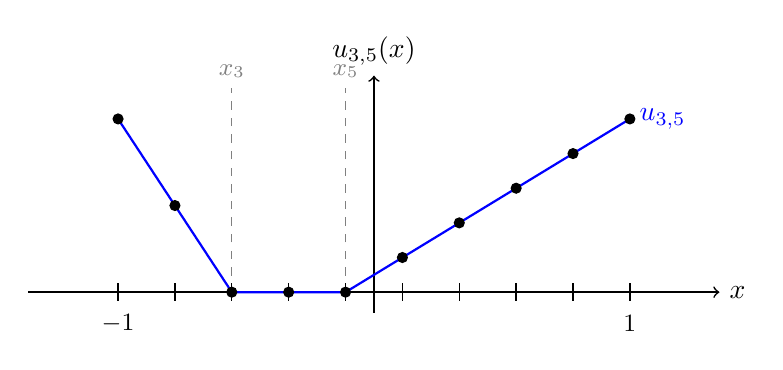
\begin{tikzpicture}[x=3.25cm,y=2.2cm] % <-- bigger overall (both axes)
        % parameters
        \pgfmathsetmacro{\d}{10}
        \pgfmathsetmacro{\a}{3}
        \pgfmathsetmacro{\b}{5}
        \pgfmathsetmacro{\xa}{-1 + 2*(\a-1)/(\d-1)}
        \pgfmathsetmacro{\xb}{-1 + 2*(\b-1)/(\d-1)}

        % axes
        \draw[->, line width=0.6pt] (-1.35, 0) -- (1.35, 0) node[right] {$x$};
        \draw[->, line width=0.6pt] (0, -0.12) -- (0, 1.25) node[above] {$u_{3,5}(x)$};

        % piecewise-linear shape of u_{3,5}
        \draw[thick, blue]
        (-1,1) -- (\xa,0) -- (\xb,0) -- (1,1);
        \node[blue, right] at (1,1) {$u_{3,5}$};

        % mark a and b breakpoints
        \draw[dashed, gray] (\xa,0) -- (\xa,1.18);
        \draw[dashed, gray] (\xb,0) -- (\xb,1.18);
        \node[gray, above] at (\xa,1.18) {\small $x_3$};
        \node[gray, above] at (\xb,1.18) {\small $x_5$};

        % grid points, ticks, and values
        \foreach \i in {1,...,10} {
                \pgfmathsetmacro{\xi}{-1 + 2*(\i-1)/(\d-1)}

                \pgfmathparse{(\i<=\a) ? (1 - (\xi+1)/(\xa+1)) : ((\i<\b) ? 0 : ((\xi-\xb)/(1-\xb)))}
                \let\yi\pgfmathresult

                \draw[line width=0.5pt] (\xi, 0.05) -- (\xi, -0.05);
                \filldraw[black] (\xi, \yi) circle (1.8pt);
            }

        % interval endpoints
        \node at (-1, -0.18) {\small $-1$};
        \node at (1, -0.18) {\small $1$};
    \end{tikzpicture}
    \caption{Example \(u_{3,5}\) on the grid \(d=10\).}
\end{figure}

The significance of this characterization is that to evaluate the worst-case performance of an estimation function $E$ and a policy $p$, it suffices to consider only the extreme points $u_{a,b}$ of $\cC_d$ instead of all convex vectors in $\cC_d$.
This is because the objective function $\Lambda_q(E, p ; v)$ is convex in $v$, and the maximum of a convex function over a convex set is attained at an extreme point of that set.